\section{Discrete-time branching}
\label{sec:discrete-branching}

We now specialise the Markov language of Section~\ref{sec:preliminaries} to the Galton--Watson process, and introduce the constant $A(p)$ that organises subcritical behaviour conditional on survival. The full analytic treatment of $A(p)$---product formulae, numerical curves, and the Koenigs obstruction---is deferred to Path~C. What is needed here is only the definition, the quasi-stationary mean it controls, and a clear statement of which parts of the picture are elementary and which are not.

\subsection{Galton--Watson process}
\label{sec:gw}

Suppose each individual produces, independently of all others, a random number of offspring $\xi$ with
\[
\pr{\xi = k} = p_k,
\qquad
k=0,1,2,\ldots,
\]
and mean $m=\mean{\xi}$; we reserve $\xx,\zz$ for process state, not for a single offspring draw. Let $\zz_n$ denote the population size in generation $n$, starting from $\zz_0=1$, so that $\mean{\zz_n}=m^n$. If $m<1$, and excluding the degenerate law concentrated at $1$, extinction is certain:
\[
\lim_{n\to\infty}\pr{\zz_n=0}=1.
\]

Write $\phi(z)=\mean{z^{\xi}}$ for the offspring \pgf, and $u_n=\pr{\zz_n=0}$ for the extinction probability by generation $n$ from a single ancestor---written ${}_1u_n$ when the initial count must be stressed. Conditioning on the first generation yields the iteration
\begin{equation}
\label{eq:iterPGF}
u_{n+1} = \phi(u_n),
\qquad
u_0=0,
\end{equation}
which is the discrete engine driving everything that follows.

\subsection{Death or division}
\label{sec:death-division}

Throughout this section we take the binary law
\begin{align*}
p_2 &= p &&\text{(division)}, \\
p_0 &= 1-p &&\text{(death)},
\end{align*}
with $p_k=0$ otherwise. Then $m=2p$, so the process is subcritical, critical, or supercritical according as $p<\tfrac12$, $p=\tfrac12$, or $p>\tfrac12$, and the unconditional mean is
\[
\mean{\zz_n} = (2p)^n.
\]
Under this law equation~\eqref{eq:iterPGF} becomes
\begin{equation}
\label{eq:unIter}
u_{n+1} = 1-p + p\, u_n^2.
\end{equation}
It is more convenient to follow survival than extinction, so let $S_n=1-u_n$ be the probability of survival to generation $n$. From \eqref{eq:unIter} one obtains
\begin{equation}
\label{eq:SnIter}
S_{n+1} = 2p\, S_n - p\, S_n^2.
\end{equation}

\subsection{Late-time survival and the constant $A(p)$}
\label{sec:Ap-def}

Restrict attention to the subcritical regime $p<\tfrac12$, where both the mean $(2p)^n$ and the survival probability $S_n$ tend to zero. Because $S_n$ is small at late times, the quadratic term in \eqref{eq:SnIter} becomes negligible relative to the linear one, and
\[
S_{n+1} \sim 2p\, S_n.
\]
The decay is therefore geometric at ratio $2p$, and the only question left is the prefactor. More precisely, there exists a constant $A(p)\in\bigl(0,\tfrac12\bigr]$, depending on $p$ but not on $n$, such that
\begin{equation}
\label{eq:lateS}
S_n \sim A(p)\, (2p)^n
\qquad\text{as }n\to\infty,
\end{equation}
or equivalently
\begin{equation}
\label{eq:Ap-limit}
A(p)
=
\lim_{n\to\infty}
\frac{S_n}{(2p)^n}.
\end{equation}
(Existence and positivity of the limit are classical for this subcritical binary process; see e.g.\ Athreya and Ney \cite{Athreya1972}. The upper bound $A(p)\leq\tfrac12$ follows because $S_1=p$ gives $S_1/(2p)=\tfrac12$, while the sequence $S_n/(2p)^n$ is decreasing, since $S_{n+1}/S_n=2p-p S_n<2p$; consequently $1/A(p)\geq 2$. The older thesis notation sometimes wrote $S_n\to A(2P)^n$ with a single letter $A$, and we standardise here on $A(p)$.)

The limit \eqref{eq:Ap-limit} is well defined and can be read off numerically by iterating \eqref{eq:SnIter}. Figure~\ref{fig:conditionalMean} plots the reciprocal ratio $(2p)^n/S_n$ against $n$ for several subcritical values of $p$: each trajectory settles to a horizontal asymptote $1/A(p)$, and that asymptote sits higher the closer $p$ comes to $\tfrac12$ from below.

\begin{figure}[ht]
\centering
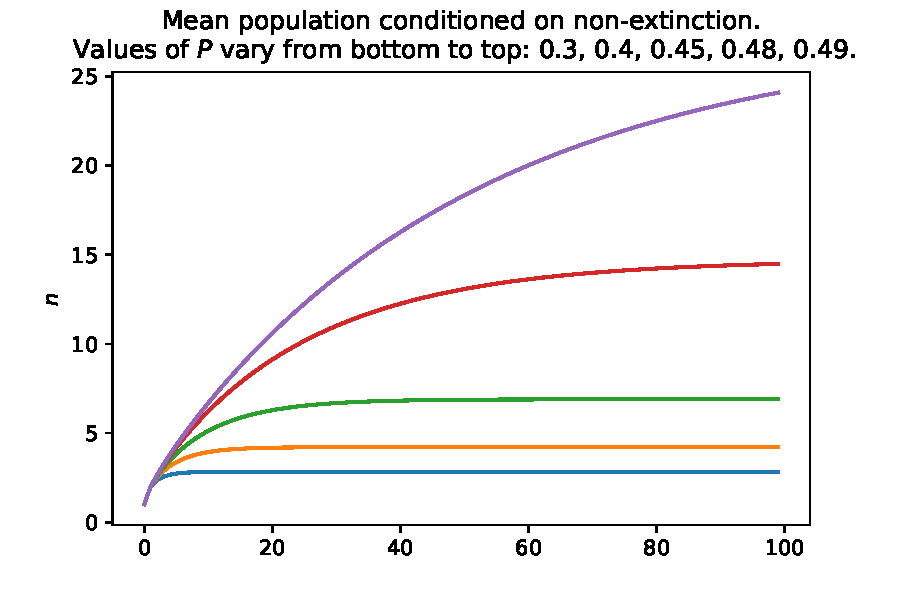
\includegraphics[width=0.8\textwidth]{figures/IMG_ch3/conditionalMean.pdf}
\caption{The ratio $(2p)^n/S_n$ against generation $n$, for subcritical division probabilities $p$. Curves nearer the top correspond to $p$ closer to criticality (e.g.\ $p=0.49$); lower curves use smaller $p$ (e.g.\ $p=0.3$). The late-time plateau is $1/A(p)$.}
\label{fig:conditionalMean}
\end{figure}

\subsection{Quasi-stationarity and conditional mean}
\label{sec:qs-discrete}

When absorption at $0$ is certain, one may still ask how the process behaves on the event of non-extinction. A limiting conditional distribution of that kind, when it exists, is called a \emph{quasi-stationary} distribution, and the plateau just seen in Figure~\ref{fig:conditionalMean} is the first sign of one.

Its mean is elementary once \eqref{eq:lateS} is granted. Decomposing the unconditional mean over the extinction event,
\[
\mean{\zz_n}
=
\pr{\zz_n\neq 0}\,
\mean{\zz_n\mid \zz_n\neq 0},
\]
gives
\[
\mean{\zz_n\mid \zz_n\neq 0}
=
\frac{(2p)^n}{S_n},
\]
which is precisely the ratio plotted above. Sending $n\to\infty$ and using \eqref{eq:lateS},
\begin{equation}
\label{eq:cond-mean}
\lim_{n\to\infty}
\mean{\zz_n\mid \zz_n\neq 0}
=
\frac{1}{A(p)}.
\end{equation}
In the subcritical death-or-division process, then, lineages that are still alive at large $n$ have expected size tending to the constant $1/A(p)$---a size scale set by the division probability alone.

\subsection{Conditional second moment and variance}
\label{sec:cond-var}

A stable conditional mean need not imply a stable spread, so it is worth pushing the same calculation one moment further. For $p<\tfrac12$ the second moment is
\begin{equation}
\label{eq:secondMoment}
\mean{\zz_n^2}
=
(2p)^n\lrb{1+\frac{1}{1-2p}}
-
(2p)^{2n}\lrb{\frac{1}{1-2p}},
\end{equation}
the derivation---via the moment generating function and a product rule along the iterate of $\phi$---being recorded in the chapter appendix. Conditioning as before and letting $n\to\infty$,
\begin{align}
\mean{\zz_n^2\mid \zz_n\neq 0}
&\to
\frac{1}{A(p)}\lrb{1+\frac{1}{1-2p}},
\label{eq:cond-second}
\\
\mathrm{Var}(\zz_n\mid \zz_n\neq 0)
&\to
\frac{1}{A(p)}\lrb{1+\frac{1}{1-2p}}
-
\frac{1}{A(p)^2}.
\label{eq:cond-var}
\end{align}
Both the conditional mean and the conditional variance therefore approach finite limits, so the late-time picture on survival is not merely a fixed mean size but a genuine quasi-stationary fluctuation scale.

\subsection{What is elementary and what is not}
\label{sec:punchline}

The constant $A(p)$ is as concrete as a limit of an explicit recurrence: it can be computed to any precision by iterating \eqref{eq:SnIter} and forming \eqref{eq:Ap-limit}. Concreteness of that kind is not the same as a closed form, and the contrast is sharp. The continuous-time birth--death process treated in the next section admits a fully closed elementary expression for the analogous reciprocal conditional mean, written directly in the rate parameters; no comparably elementary closed form for $p\mapsto A(p)$ on $p\in[0,\tfrac12)$ is available. The obstruction, and the usable representations that survive it, are the subject of Path~C. For the rest of Path~A it is enough to treat $A(p)$ as a well-defined, numerically accessible factor that converts a decaying survival probability into a stable conditional mean $1/A(p)$.
